
%(BEGIN_QUESTION)
% Copyright 2012, Tony R. Kuphaldt, released under the Creative Commons Attribution License (v 1.0)
% This means you may do almost anything with this work of mine, so long as you give me proper credit

Assuming all three alternators are equally sharing the load in this power system, that the primary:secondary turns ratio in the three-phase transformer is 30:1, that the power factor is 1 throughout the system, and that all disconnect switches are closed, calculate the following:

$$\includegraphics[width=15.5cm]{i01046x01.eps}$$

\begin{itemize}
\item{} Line voltage of the generator bus = \underbar{\hskip 50pt} volts
\vskip 10pt
\item{} Line voltage of the load bus = \underbar{\hskip 50pt} volts
\vskip 10pt
\item{} Line current at each alternator = \underbar{\hskip 50pt} amps 
\vskip 10pt
\item{} Total power transferred in this system with all loads running = \underbar{\hskip 50pt} kilowatts 
\end{itemize}

\underbar{file i01046}
%(END_QUESTION)





%(BEGIN_ANSWER)

\noindent
{\bf Partial answer:}

\vskip 10pt

The line voltage at the generator bus is given to us by the alternator rating of 4160 volts.  Unless otherwise specified, the voltage or current rating of a three-phase device is always a {\it line} quantity.

%(END_ANSWER)





%(BEGIN_NOTES)

\begin{itemize}
\item{} Line voltage of the generator bus = \underbar{\bf 4160} volts ({\it given})
\vskip 10pt
\item{} Line voltage of the load bus = \underbar{\bf 240.18} volts
\vskip 10pt
\item{} Line current at each alternator = \underbar{\bf 3.398} amps 
\vskip 10pt
\item{} Total power transferred in this system with all loads running = \underbar{\bf 73.46} kilowatts 
\end{itemize}

\vskip 10pt

The load bus receives its power through the step-down transformer, with 30:1 ratio between primary and secondary windings.  Each primary winding sees the full 4160 VAC of the generator bus, because those windings are in a delta configuration.  Thus, each secondary winding will output $1 \over 30$ of that, or 138.67 volts.  Since the secondary windings are connected together in a wye configuration, the line voltage at the load bus will be 240.18 volts.

\vskip 10pt

The next logical calculation to perform is total power, because we cannot calculate alternator line current until we know how much power they're sourcing.  The two 35 HP motors are easy: 28.075 kW each.  Thus, the total motor load is 56.15 kW.  Power dissipated by the delta-connected resistor load is the sum of each resistor's dissipation (240.18 volts across 10 ohms), which is 3 $\times$ 5768.5 watts, or 17305.6 watts.  Since power is a scalar quantity, we know all power dissipations in a system must simply add to make the total.  Therefore, the total power in this system is 73.456 kW.

\vskip 10pt

If we now treat the three alternators as a single power source (at a line voltage of 4160 volts), the total power dissipation of 73.456 kW equates to a total line current of 10.195 amps.  Split evenly among three alternators, the line current for each alternator must be one-third of this, or 3.398 amps.

%INDEX% Electronics review: 3-phase electrical power 
%INDEX% Electronics review: AC transformer circuit

%(END_NOTES)


